\documentclass[
  bibliography=totoc,     % Literatur im Inhaltsverzeichnis
  captions=tableheading,  % Tabellenüberschriften
  titlepage=firstiscover, % Titelseite ist Deckblatt
]{scrartcl}

% LaTeX2e korrigieren.
\usepackage{fixltx2e}
% Warnung, falls nochmal kompiliert werden muss
\usepackage[aux]{rerunfilecheck}

% deutsche Spracheinstellungen
\usepackage{polyglossia}
\setmainlanguage{german}

% unverzichtbare Mathe-Befehle
\usepackage{amsmath}
% viele Mathe-Symbole
\usepackage{amssymb}
% Erweiterungen für amsmath
\usepackage{mathtools}

% Fonteinstellungen
\usepackage{fontspec}
\defaultfontfeatures{Ligatures=TeX}

\usepackage[
  math-style=ISO,    % \
  bold-style=ISO,    % |
  sans-style=italic, % | ISO-Standard folgen
  nabla=upright,     % |
  partial=upright,   % /
]{unicode-math}

\setmathfont{Latin Modern Math}
\setmathfont[range={\mathscr, \mathbfscr}]{XITS Math}
\setmathfont[range=\coloneq]{XITS Math}
\setmathfont[range=\propto]{XITS Math}
% make bar horizontal, use \hslash for slashed h
\let\hbar\relax
\DeclareMathSymbol{\hbar}{\mathord}{AMSb}{"7E}
\DeclareMathSymbol{ℏ}{\mathord}{AMSb}{"7E}

% richtige Anführungszeichen
\usepackage[autostyle]{csquotes}

% Zahlen und Einheiten
\usepackage[
  locale=DE,                   % deutsche Einstellungen
  separate-uncertainty=true,   % Immer Fehler mit \pm
  per-mode=symbol-or-fraction, % m/s im Text, sonst Brüche
]{siunitx}

% chemische Formeln
\usepackage[version=3]{mhchem}

% schöne Brüche im Text
\usepackage{xfrac}

% Floats innerhalb einer Section halten
\usepackage[section, below]{placeins}
% Captions schöner machen.
\usepackage[
  labelfont=bf,        % Tabelle x: Abbildung y: ist jetzt fett
  font=small,          % Schrift etwas kleiner als Dokument
  width=0.9\textwidth, % maximale Breite einer Caption schmaler
]{caption}
% subfigure, subtable, subref
\usepackage{subcaption}

% Grafiken können eingebunden werden
\usepackage{graphicx}
% größere Variation von Dateinamen möglich
\usepackage{grffile}

% Standardplatzierung für Floats einstellen
\usepackage{float}
\floatplacement{figure}{htbp}
\floatplacement{table}{htbp}

% schöne Tabellen
\usepackage{booktabs}

% Seite drehen für breite Tabellen
\usepackage{pdflscape}

% Literaturverzeichnis
\usepackage{biblatex}
% Quellendatenbank
\addbibresource{lit.bib}
\addbibresource{programme.bib}

% Hyperlinks im Dokument
\usepackage[
  unicode,
  pdfusetitle,    % Titel, Autoren und Datum als PDF-Attribute
  pdfcreator={},  % PDF-Attribute säubern
  pdfproducer={}, % "
]{hyperref}
% erweiterte Bookmarks im PDF
\usepackage{bookmark}

% Trennung von Wörtern mit Strichen
\usepackage[shortcuts]{extdash}

\author{
  AUTOR A%
  \texorpdfstring{
    \\
    \href{mailto:authorA@udo.edu}{authorA@udo.edu}
  }{}%
  \texorpdfstring{\and}{, }
  AUTOR B
  \texorpdfstring{
    \\
    \href{mailto:authorB@udo.edu}{authorB@udo.edu}
  }{}
}
\publishers{TU Dortmund – Fakultät Physik}


\title[Toolbox 2019]{Toolbox-Workshop 2019}
\subtitle{Python, Unix, Make, Git, \LaTeX{}}
\date{23.~September – 4.~Oktober 2019}
\institute[Pep et al.\ e.V.]{
\includegraphics[height=2cm]{logos/pep.pdf}}
\author[Toolbox-Team]{}

\begin{document}

\maketitle

\begin{frame}{Ziel}
  \setlength\parskip{3ex}
  \huge
  Wir machen euch das Praktikum so einfach, wie möglich.

  Auswerten mit modernen Methoden.

  Von Anfang an ein bewährter Weg.

  Auch für die Bachelorarbeit wichtig.
\end{frame}

\begin{frame}
  \vspace{2cm}
  \begin{center}
    \huge Praktikums-Versuche richtig auswerten!\\
    23. – 27.~September 2019, 13–17~Uhr, CT-ZB ZE01
  \end{center}
  \begin{tikzpicture}[remember picture, overlay]
    \tikzset{shift={(current page.center)}}
    \node[anchor=center] at (-3,2) {%
      
\includegraphics[height=1.5cm]{logos/python.pdf}%
    };
    \node[anchor=center] at (3,2) {%
      
\includegraphics[height=1.25cm]{logos/git.png}%
    };
    \node[anchor=center] at (4,-2) {%
      
\includegraphics[height=1cm]{logos/numpy.png}%
    };
    \node[anchor=center] at (-2.5,-2) {%
      
\includegraphics[height=1cm]{logos/matplotlib.png}%
    };
    \node[anchor=center] at (0,-3.5) {%
      
\includegraphics[height=0.75cm]{logos/uncertainties.png}%
    };
  \end{tikzpicture}
\end{frame}

\begin{frame}[plain]
  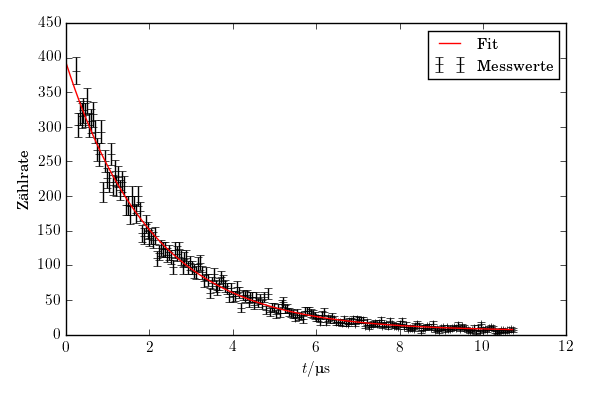
\includegraphics[width=\textwidth]{../python/build/muon_plot.png}
\end{frame}

\begin{frame}
  \begin{center}
    \huge Wissenschaftliche Arbeiten verfassen mit \\[0.5\baselineskip]
    \textrm{\fontsize{80}{120}\selectfont\LaTeX{}}\\[0.5\baselineskip]
    30.~September–04.~Oktober 2019, 13–17~Uhr, CT-ZB ZE01\\
    \textcolor{red!70!black}{Am 2.~Oktober in Chemie HS03}
  \end{center}
\end{frame}

\begin{frame}{Vorbereitung}
  \begin{center}
    \huge
    Auf der Fachschaftsmailingliste eintragen \\
    \url{https://mailman.tu-dortmund.de/mailman/listinfo/stud.physik}\\[0.5\baselineskip]
    Software installieren\\
    → \textcolor{blue!70!black}{\url{https://toolbox.pep-dortmund.org/install}}\\[0.5\baselineskip]
    Umfrage ausfüllen\\[0.5\baselineskip]
    Laptops mitbringen / uns ansprechen
  \end{center}
\end{frame}
\begin{frame}{Installation}
  \huge
  Falls es Probleme bei der Installation gibt oder ihr Linux installieren wollt:\\[0.5\baselineskip]
  \begin{enumerate}
    \item Mail an \href{mailto:toolbox-pep-dortmund@googlegroups.com}{toolbox-pep-dortmund@googlegroups.com}
    \item Im Büro vorbeikommen (CP-03-156/CP-01-178)
    \item Montag 23.09.2019: ab 9:00 betreutes Installieren in CP-03-150
  \end{enumerate}
\end{frame}
\begin{frame}
  \Huge\centering
  \textcolor{red!70!black}{Fragen?}
\end{frame}
\end{document}
